\section{Figures}

\begin{figure}[h!]
	\centering
	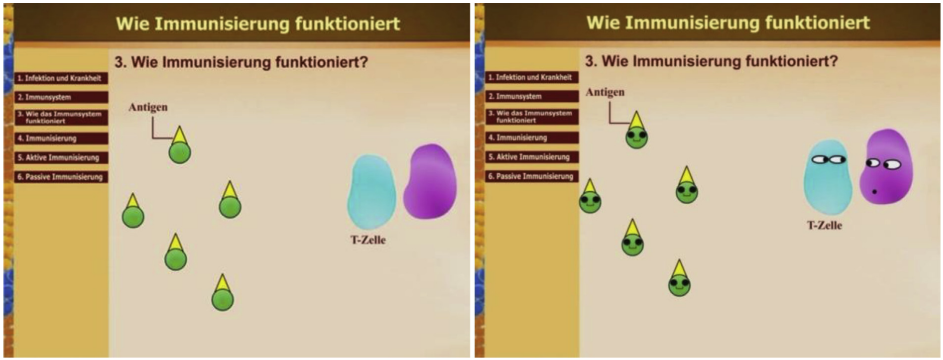
\includegraphics[width=1\linewidth]{graphics/anthropomorphisms}
	\caption{Screenshots of the learning program in the neutral version (left) and the positive version with anthropomorphisms (right). Taken from \cite{Park2015}}
	\label{fig:anthropomorphisms}
\end{figure}

\begin{figure}
	\centering
	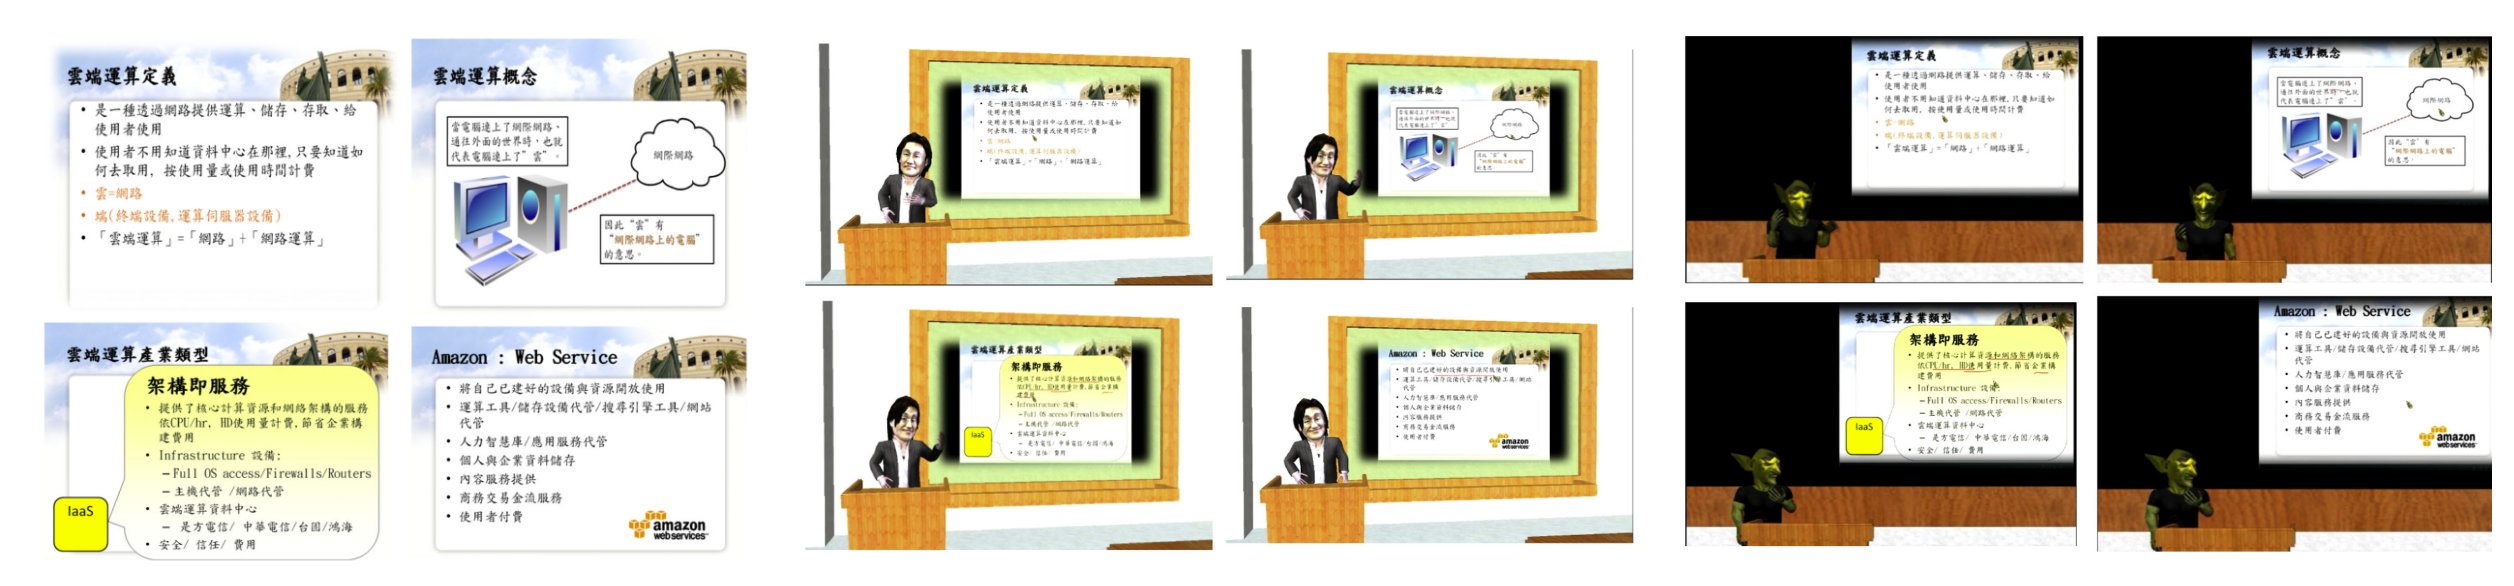
\includegraphics[width=1\linewidth]{graphics/The_effects_of_multimedia_instructional_materials}
	\caption{The effects of various multimedia instructional materials. Left to right - control group interface, experimental Group I interface (human-like animated character) and experimental Group II interface (monster-like animated character). From \cite{Lee2014}}
	\label{fig:theeffectsofmultimediainstructionalmaterials}
\end{figure}

\begin{figure}
	\centering
	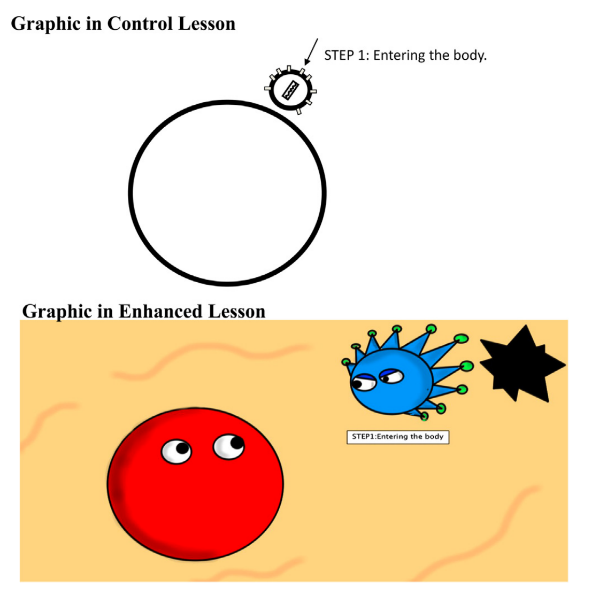
\includegraphics[width=0.7\linewidth]{graphics/Benefits_of_emotional_design_in_multimedia_instruction}
	\caption{Graphics from control and enhanced group. From \cite{Mayer2014}}
	\label{fig:benefits-bio-lesson}
\end{figure}	